%-- Add sections and your outline will be created automatically --%
\section{Rotating periodic channel}

% Frame starts a new slide
\begin{frame}
    \frametitle{Rotating periodic channel}
\begin{itemize}
\item Domain: Unit square, periodic in zonal direction.
\item Boundary conditions: No-slip at the North and South boundaries.
\item Coriolis applied.
\item Forcing applied by a Python function.
\item The flow is driven by a velocity source term:
\begin{equation*}
  \vec{F}=
  \begin{bmatrix}
    y^3 \\
    0
  \end{bmatrix}
\end{equation*}
\item Parameters are chosen such that the solution converges to a steady state with a known analytical solution.
\end{itemize}
\end{frame}
%
\begin{frame}
    \frametitle{Rotating periodic channel}
\begin{figure}
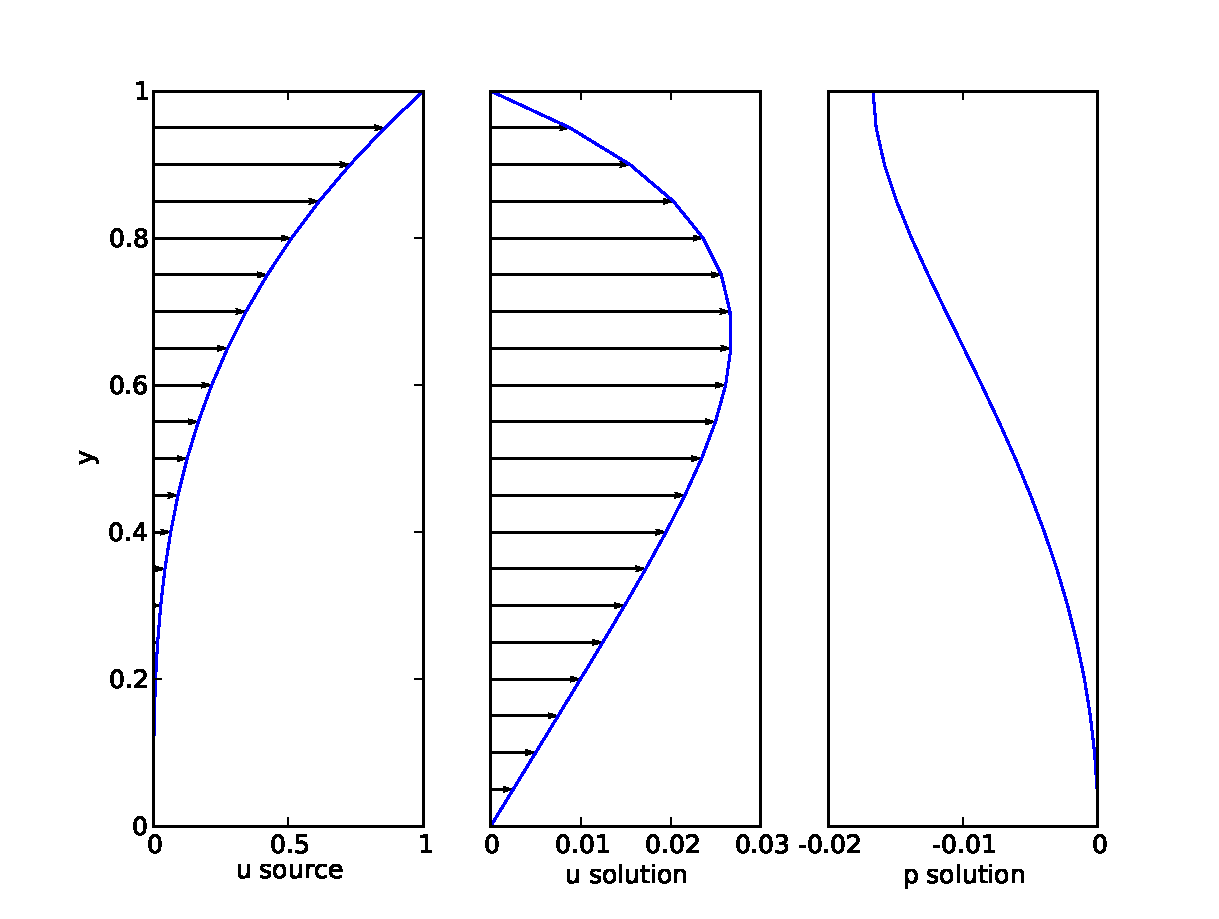
\includegraphics[width=0.6\textwidth]{./rotating_channel/analytic_solution}
\caption{Velocity forcing term and analytic solutions for velocity and pressure.  Each of these quantities are constant in the x direction.}
\end{figure}
\end{frame}
%
\begin{frame}
    \frametitle{Rotating periodic channel}
\begin{figure}
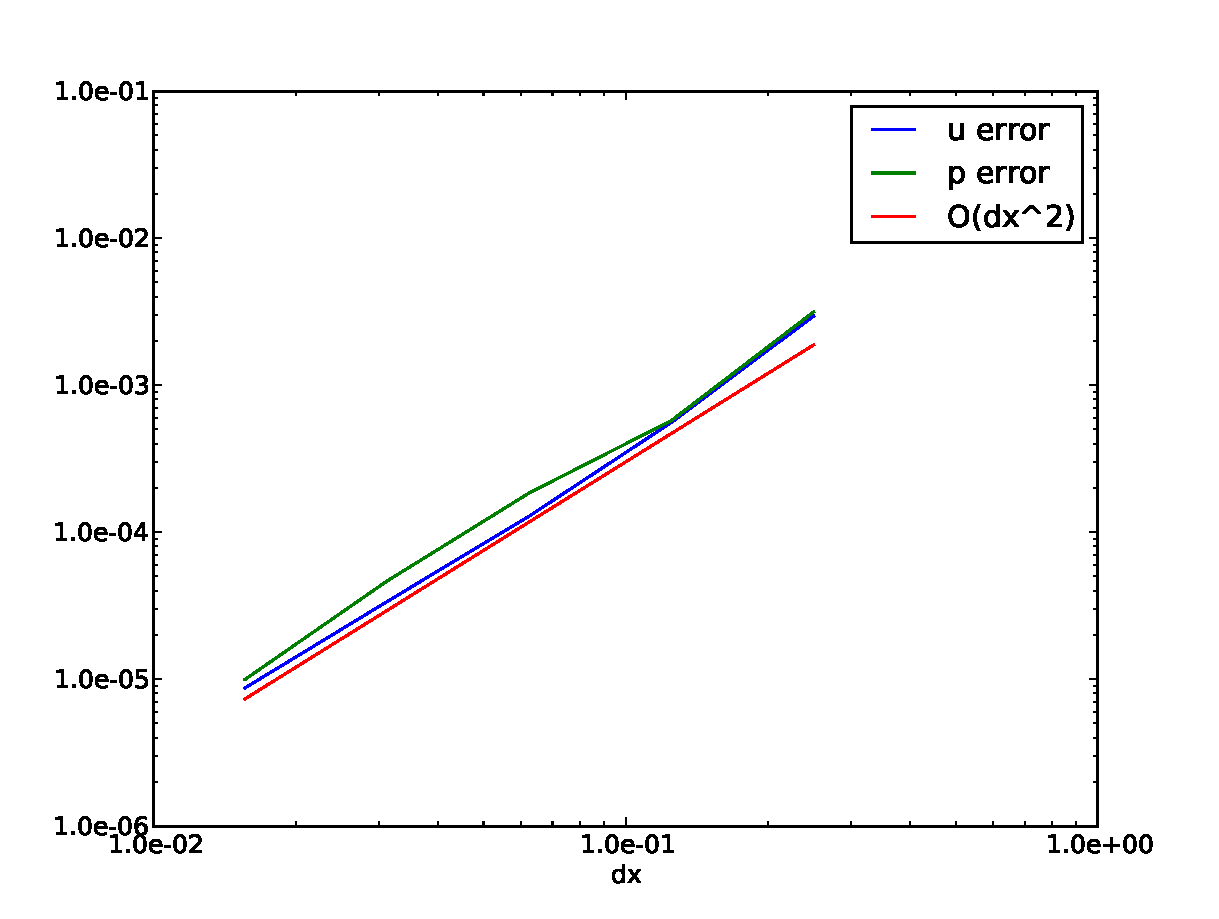
\includegraphics[width=0.6\textwidth]{./rotating_channel/convergence}
\caption{Error in the pressure and velocity solutions as a function of mesh resolution.}
\end{figure}
\end{frame}
%
\begin{frame}
    \frametitle{Rotating periodic channel, exercises}
\begin{itemize}
\item Understand the use of analytic forcing functions in Fluidity using Python (e.g. take a look at \url{channel_tools.py} and \url{plot_theory}).
\end{itemize}
\end{frame}

